\begin{center}
\begin{figure}[h!]
\begin{center}
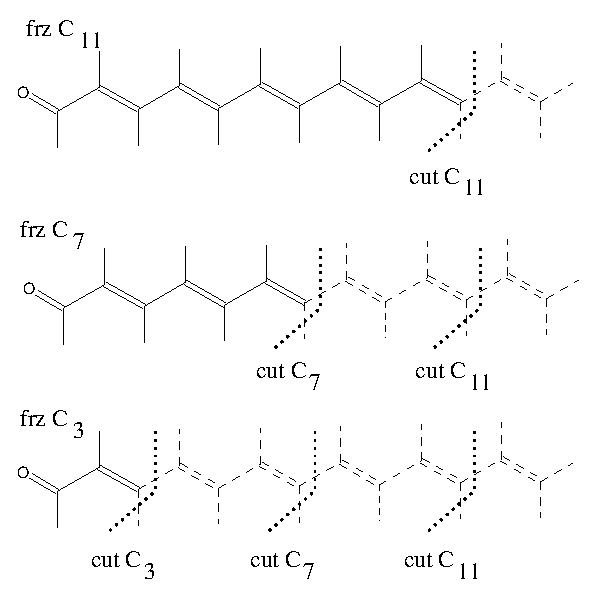
\includegraphics[width=8cm,keepaspectratio]{02_localization/images/C13-selection.eps}
\end{center}
\caption{\footnotesize C$_{13}$ polyenal molecule. Freeze and cut strategy
and labels follow the analogy with shorter chain polyenals. Localized
orbitals expressed on atoms of the dashed line framework are frozen.
Dotted lines depict the cut seam.  }
\label{fig:C13-selection}
\end{figure}
\end{center}
